%!TEX root = ../../novoIndex.tex

As \emph{Smart} TVs são o resultado da evolução tecnológica junto aos aparelhos de televisão domésticos. Possuem capacidades interativas ligadas à internet, acesso a conteúdo online, \emph{e-commerce} de conteúdo televisivo, navegação web e acesso a redes sociais. Estes aparelhos podem ser equipados com câmeras e microfones e são capazes de transmitir conteúdo 2D e 3D \cite{samsung:smarttv,perakakis2015proposed}.

O principal diferencial no tocante ao hardware entre \emph{Smart} TVs e as antigas tecnologias LED e LCD TV reside na conexão com a internet, que pode ser realizada via módulo Wi-Fi ou Ethernet \cite{differencebetween,tomsguid:everythingsmart}. Para promover esta conexão e posterior interação com o usuário, estas televisões utilizam os mesmos sistemas operacionais e conjuntos de aplicativos que computadores ou \emph{smartphones} convencionais, em especial mencionam-se navegador web e diversos aplicativos.

É possível também que \emph{Smart} TVs exibam conteúdo de mídia transmitido a partir de \emph{smartphones}, \emph{players} de mídia ou computadores conectados na mesma rede Wi-Fi, conforme o padrão de compartilhameto de mídia DLNA (\emph{Digital Living Network Alliance}) \cite{michele2014watch,shin2013smart,perakakis2015proposed,whatisasmarttv}. Muitos modelos destes televisores também possuem ferramentas para o reconhecimento de comandos de voz, possibilitando funcionalidades como troca e busca de canais, controle de volume, etc. Este controle de voz costuma também estar integrado com funções das casas inteligentes, tendência da Internet das Coisas \cite{tomsguid:everythingsmart}.

A Figura \ref{fig:smart_samsung} exibe um diagrama representativo dos elementos que compõem uma \emph{Smart} TV. As legendas para os números apresentados na imagem estão na Tabela \ref{tab:smart}. Dentre os diversos fabricantes destes dispositivos, em nível mundial destacam-se as marcas Hisence, LG, Panasonic, Phillips. Samsung, Sharp, Sony, TCL, Toshiba e Vizio \cite{tomsguid:everythingsmart}.

\begin{figure}[!ht]
	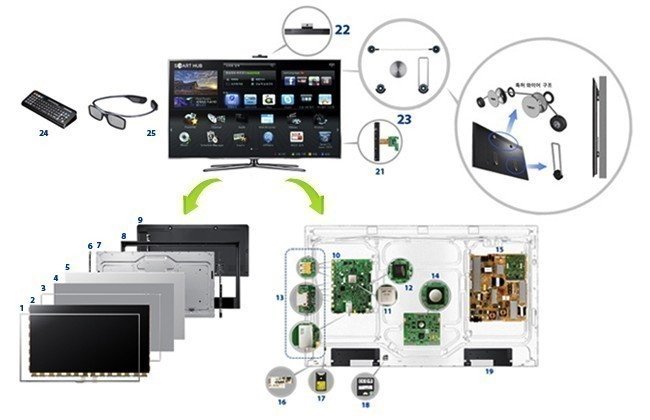
\includegraphics[width=\textwidth]{img/smart_samsung.jpg}
	\caption{Diagrama representativo de uma \emph{Smart} TV e seus componentes \cite{samsung:smarttv}. Ver legenda dos componentes na Tabela \ref{tab:smart}.}
	\label{fig:smart_samsung}
\end{figure}

\begin{table}[!ht]
	\centering
	\caption{Legenda dos componentes citados na Figura \ref{fig:smart_samsung}.}
	\label{tab:smart}
	\scalefont{0.77}
	\begin{tabular}{c l  c l}
		\toprule
		\textbf{Número} & \textbf{Descrição} & \textbf{Número} & \textbf{Descrição}\\
		\midrule
		1 & Moldura & 13 & Sintonizador, 4 portas HDMI e 3 portas USB \\
		2 & Painel de cristal negro (célula) & 14 & 3D \emph{Hyper Real Engine}\\
		3 & Molde da moldura intermediária & 15 & Placa de Alimentação \\
		4 & Folha óptica & 16 & Sensor de luz\\
		5 & LGP -- \emph{Light Guide Plate} & 17 &  Módulo \emph{bluetooth} \\
		6 & LED & 18 & Módulo Wi-Fi\\
		7 & Chassi traseiro & 19 & Auto-falantes \\
		8 & Cobertura intermediária & 20 & Suporte quadrangular\\
		9 & Cobertura traseira & 21 & Botão \emph{touch} operacional\\
		10 & Placa de circuito principal (Placa mãe) & 22 & Câmera\\
		11 & \emph{Smart Real Engine} & 23 & Suporte de parede \\
		12 & \emph{Speed Backlite Engine} & 24 & Controle remoto QWERTY\\
		   &  & 25 & Óculos 3D \\
		\bottomrule
	\end{tabular}
\end{table}

As aplicações disponíveis para \emph{Smart} TVs são diversas, permitindo, por exemplo, o acesso a conteúdo de programas e também a informações esportivas, como é comum no caso do futebol. Um exemplo de aplicação disponível para \emph{Smart} TVs é a disponibilizada desde 2016 pela emissora aberta SBT, vide Figura \ref{fig:sbt_app}. Este aplicativo contém novelas, programas e outras atrações disponibilizadas pela emissora que podem ser assistidos \emph{on demand} \cite{sbt:tvconectada}. Outros exemplos compreendem os aplicativos de \emph{streaming}, tais como Netflix, Amazon Prime Video, Hulu e Pandora \cite{canaltech:streaming}.

\begin{figure}[!ht]
	\centering
	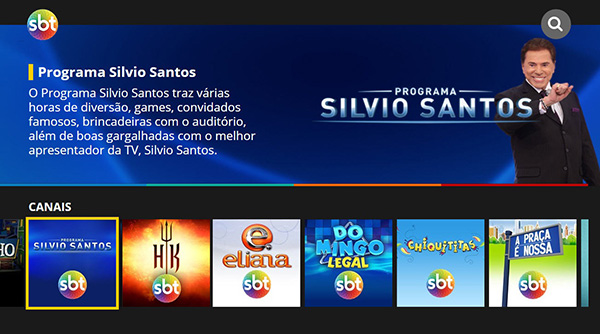
\includegraphics[width=\textwidth]{img/sbt_app.jpg}
	\caption{Aplicativo SBT. Fonte: \cite{sbt:tvconectada}}
	\label{fig:sbt_app}
\end{figure}

Segundo a Pesquisa Nacional por Amostra de Domicílios (PNAD) realizada pelo IBGE em 2015, foi observado um total de $103$ milhões de aparelhos de televisões em residências e pontos comerciais, das quais $16$ milhões são de \emph{Smart} TVs. A pesquisa detalha que $94\%$ destas \emph{Smart} TVs foram adquiridas entre $2014$ e $2015$. Os números mostram um posterior aumento nas vendas de aparelhos televisores deste tipo, representando $68,2\%$ do total de televisores vendidos no primeiro semestre de $2017$ \cite{pnad2015}.

Há muitos benefícios resultantes do uso de \emph{Smart} TVs quando comparadas aos aparelhos convencionais. Em especial, cita-se o aumento da qualidade na transmissão, a utilização de aplicativos diversos e a possibilidade de acesso à conteúdo \emph{online} e \emph{on demand}, gratuitos ou mediante assinaturas. Além destes benefícios, cuja maioria é resultante da conectividade com a internet, outros fatores têm justificado o aumento das vendas e do interesse do público consumidor pelas \emph{Smart} TVs, tais como o encerramento da transmissão de sinal analógico da televisão aberta, a Copa do Mundo 2018 e a tecnologia 4K \cite{leiajabuscasmart,correiopnad,estadao:explosaovideosonline}.

Apesar da grande disponbilidade de conteúdo nas \emph{Smart} TVs, é imprescindível levar em conta as restrições e recomendações deste conteúdo para o público alvo a que se destina. Neste sentido, a próxima seção detalha as políticas vigentes de classificação indicativa de conteúdo televisivo.
